% !TeX program = xelatex

\documentclass[final]{cubedoc}

\title{PCB Handbook}
\docid{AcubeSAT-OBC-G-009}
\author{Theodoros Katzalis}

\changelog{13/08/2019}{0.1}{INTERNALLY RELEASED}{Initial revision}
\changelog{15/08/2019}{0.2}{INTERNALLY RELEASED}{Remove WIP from title and fix some typos}

\usepackage{wrapfig}
\usepackage{subcaption}
\usepackage{hyperref}


\begin{document}
	
	\section{Preface}
	%What is the purpose of this report? How to read this report? What sections you can skip? If you are in x subsystem you might be find useful these y sections…
	%Learning materials are spread throughout the report, but if you want a synopsis you can found it in the end of this report! In “what is a PCB ?”, where the fabrication process is explained, it is focused on how professional manufacturers do their jobs and not how you can do it yourself. On the other hand, a DIY part would be very nice to have in the upcoming versions!Sometimes I was trying to use simple words for better comprehension just to feel what I was trying to say, so bare with me!!
	
	The purpose of this report is to make the reader feel familiar with the PCB fabrication  and to give an insight about the PCB considerations/guidelines you need to take into account when the time for design comes. So, it is divided in two main parts: \textbf{"What is a PCB?"} and \textbf{"How to design a PCB?"} In the first part, the fabrication process is explained and it is focused on how manufacturers in the PCB industry do their jobs (On the other hand, a Do It Yourself section would be very nice to have). The second part isn't oriented on how to use a CAD tool, but implies the potential problems in signal integrity and the countermeasures. If you don't have time to read thoroughly the whole report, then you should check the the \autoref{subsec:techniques} (PCB Layout techniques) and \autoref{subsec:thumb} (Rules of thumb).
	%How I learned about PCB, where tou could find useful information + just design, print, DIY, play, do stuff!
	
	\section{Disclaimer}
	This report is marked as \textbf{W}ork \textbf{I}n \textbf{P}rogress, because a lot more should be added in order to have a well completed-organized-detailed guide for PCB design. Although, I think that the the word “complete” is very uncertain and undefined, but it means that a lot more things will be discovered throughout the PCB journey, so everyone can share their personal knowledge and experience. Also, due to time constraints, some topics aren’t described in-depth. It is worth mentioning that we won’t reinvent the wheel, but we are collecting information to provide an orientation/guidance to those who thrive to design a PCB. I hope that the current version is adequate to develop an insight about PCBs and the mindset for designing quite efficiently the AcubeSAT’s boards, in the time remaining. Of course, more questions and clarifications can be made individually with the AcubeSAT’s members that have some experience in PCB design. And...of course, for the time being, this report is for internal release. 
	
	\section{What is a PCB?}
	
	\begin{wrapfigure}{R}{0.4\textwidth}
		\centering
		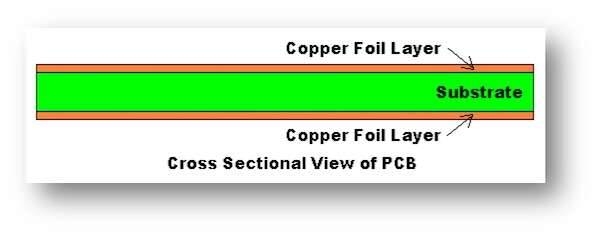
\includegraphics[width=0.4\textwidth]{assets/simple_2_layer_PCB.jpg}
		\caption{2-layer PCB}
		\label{fig:1}
	\end{wrapfigure}
	
	PCB is a \textbf{P}rinted \textbf{C}ircuit \textbf{B}oard and it is  a “sandwich” of conductive and non-conductive materials in order to control the electrical flow/signals between electrical components. It’s the place, where these components can be hosted and communicate with each other and it can be described as their mechanical and electrical support. PCBs have developed a lot throughout the years: The irreversible development of modern electronics has been increasingly pushing them towards such demands as miniaturization, light weight, high speed, better functionality and reliability, and longer lifetime. Just check the figure 2 and you will feel how time change things!
	
	\begin{figure}[h!]
		\centering
		\begin{subfigure}{.5\textwidth}
			\centering
			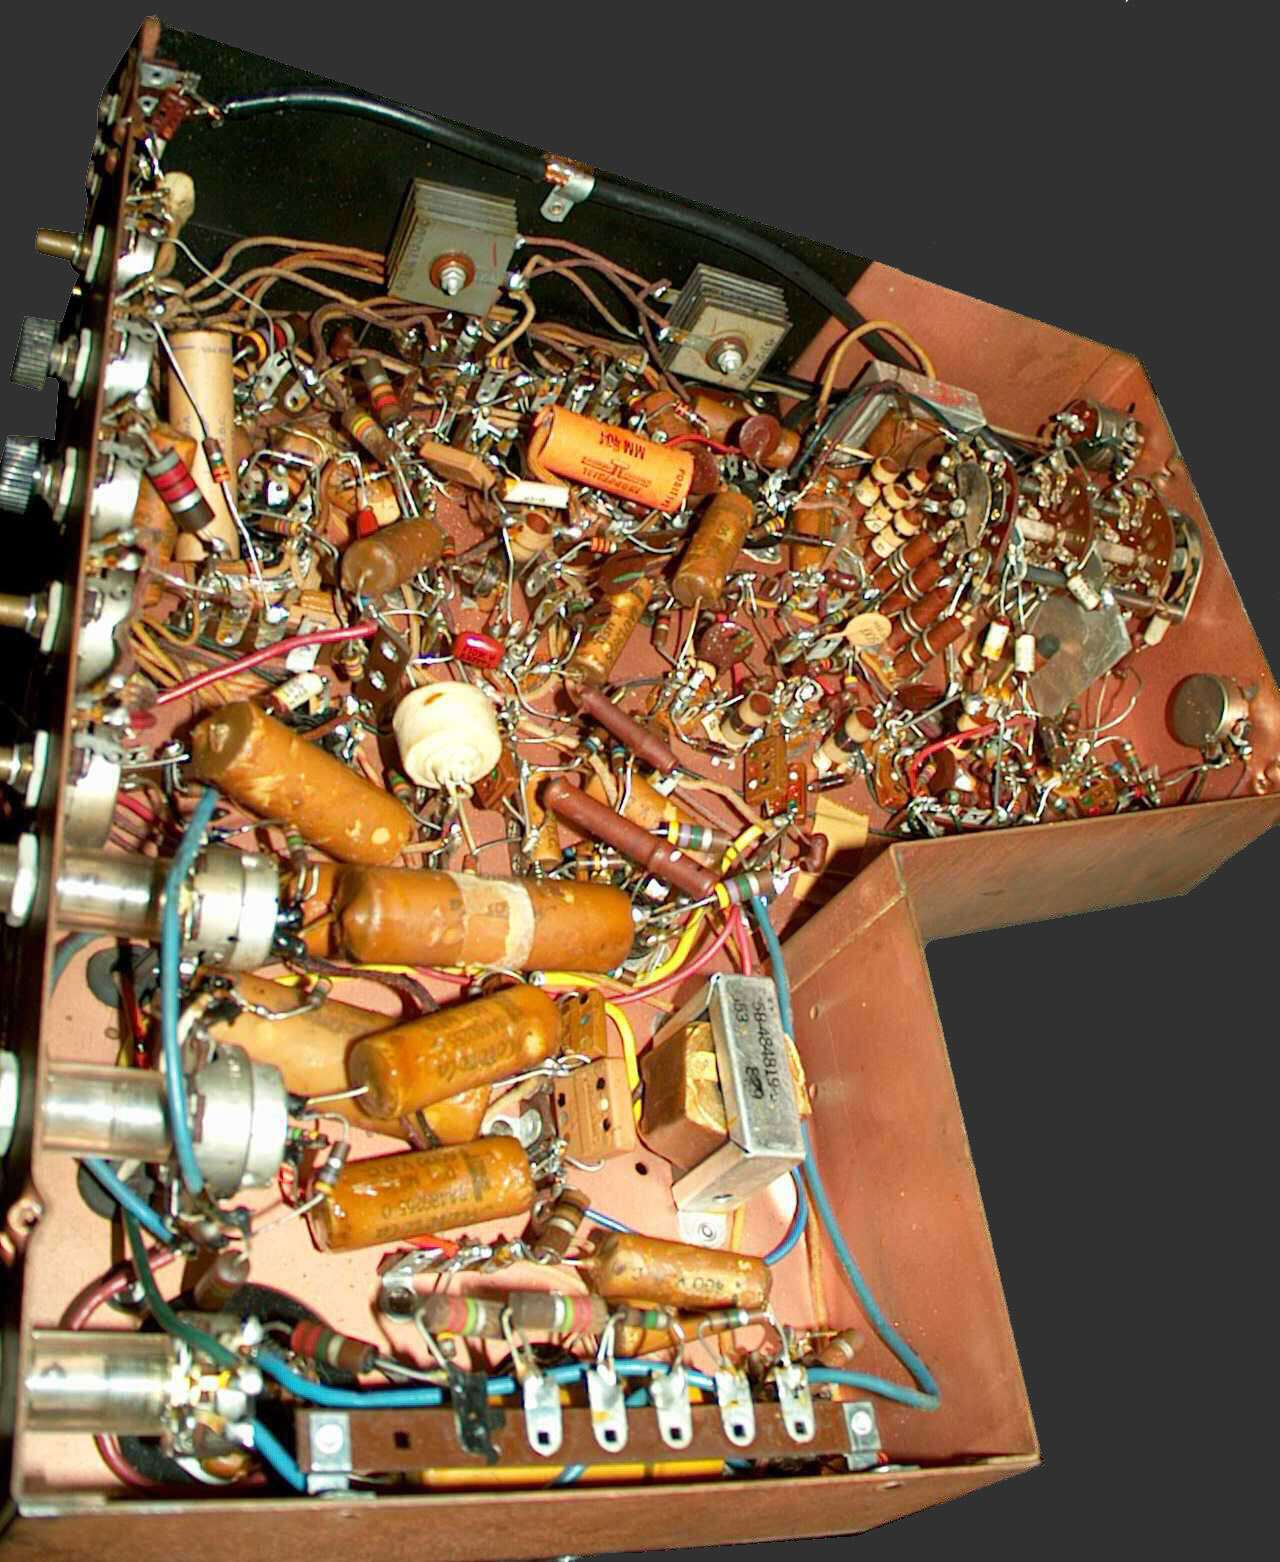
\includegraphics[height=0.25\textheight, width=.8\textwidth]{OBC/AcubeSAT-OBC-G-009_No2/assets/old_school_TV_PCB.jpg}
			\label{fig:sub1}
		\end{subfigure}%
		\begin{subfigure}{.5\textwidth}
			\centering
			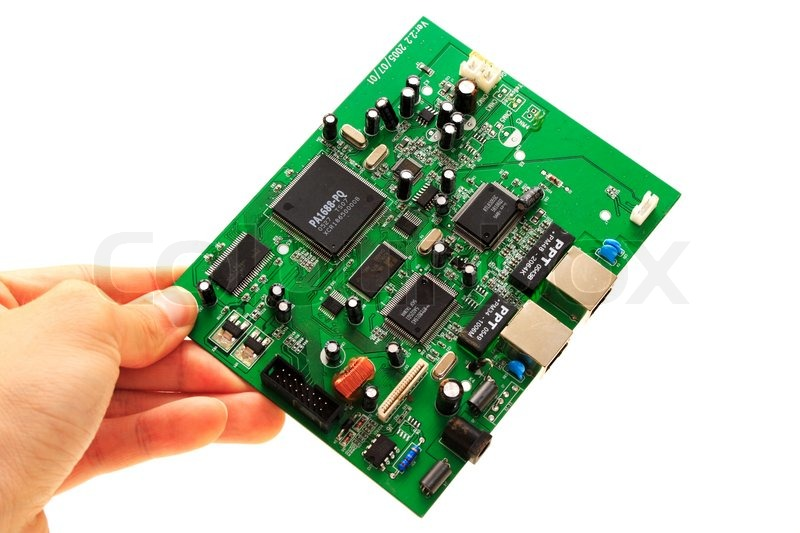
\includegraphics[height=0.25\textheight, width=.8\textwidth]{OBC/AcubeSAT-OBC-G-009_No2/assets/modern_PCB.jpg}
			\label{fig:sub2}
		\end{subfigure}
		\caption{An old school TV's PCB on the left and a modern PCB on the right}
		\label{fig:test}
	\end{figure}
	
	\subsection{Materials}
	
	As mentioned earlier, PCB is mainly a stack of conductive and non-conductive materials.
	
	\begin{itemize}
		\item conductive: we are referring to \textbf{copper foils}
		\item non-conductive: we are referring mostly to \textbf{FR-4} and it used as the dielectric substrate (separation of the copper foils). But for the non- conductive materials there is a huge variety and it depends on the application.
	\end{itemize}
	
	To be more precise, copper clad laminate, abbreviated to CCL, is a type of base material of PCBs. With glass fiber or wood pulp paper as reinforcing material, a CCL is a type of product through lamination with copper clad on either one side or both sides of reinforcing material after being soaked in resin (more info about the materials used in PCB can be found \href{https://www.pcbcart.com/article/content/copper-clad-laminate.html}{here} and \href{https://www.pcbcart.com/pcb-capability/pcb-materials.html}{here}). You can also check \href{https://www.eurocircuits.com/technical-specifications-of-all-eurocircuits-prototype-small-volume-services-european-origin/}{the technical specifications of Eurocircuits}, the manufacturer, that cooperates with Prisma!
	
	\begin{figure}[h]
		\centering
		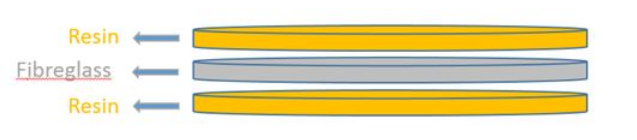
\includegraphics[width=0.8\textwidth,height=0.8\textheight,keepaspectratio]{assets/fiberglass_resin.png}
		\caption{Uncured FR-4}
	\end{figure}
	
	Is everything related about materials include in this section? Actually, no! In PCB fabrication, more complementary processes are required (\autoref{subsec:complementary}).
	
	But, first of all let’s visualize and comprehend the structure and the manufacturing process of these magic boards! Printed Circuit Boards can have different numbers of layers and sides, but can also come in changing inflexibilities. 
	
	\subsection{Inflexibility}
	In terms of inflexibility, there are three main types. The three types are 1) rigid, 2) flex and 3) rigid-flex PCBs:
	
	\subsubsection{Rigid}
	Most customers usually think of inflexible PCBs when they image a circuit board. Rigid printed circuit boards use a solid, rigid substrate material like fiberglass that remains the board from twisting. A motherboard within the tower of a computer is the best example of an inflexible PCB.
	
	\subsubsection{Flex}
	Generally, the substrate in a flexible board is a flexible plastic. This fundamental material permits the board to fit into forms that inflexible boards cannot & to turn or shift during use without harmful the circuits on the printed circuit board. Though flex boards tend to charge more to intend and create than rigid PCBs, they come with a number of advantages. For instance, they can restore heavy or bulky wiring in superior gear like \textbf{satellites}, where weight & space matter. Flex boards can also come in three formats, namely single sided, double-sided or multi-layer formats.
	
	\subsubsection{Rigid-Flex}
	Rigid flex boards merge technology from both flexible and rigid circuit boards. An easy rigid-flex boards comprises of a rigid circuit board that joints to a flex circuit board. These boards can be more compound if design requests demand.
	
	\begin{figure}[h!]
		\centering
		\begin{subfigure}{.3\textwidth}
			\centering
			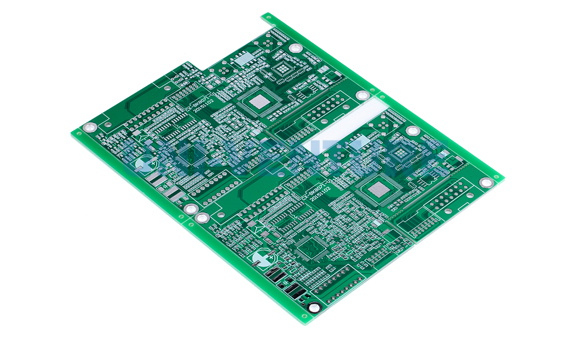
\includegraphics[height=0.2\textheight, width=.8\textwidth]{OBC/AcubeSAT-OBC-G-009_No2/assets/rigid.jpg}
			\label{fig:sub1}
		\end{subfigure}%
		\begin{subfigure}{.3\textwidth}
			\centering
			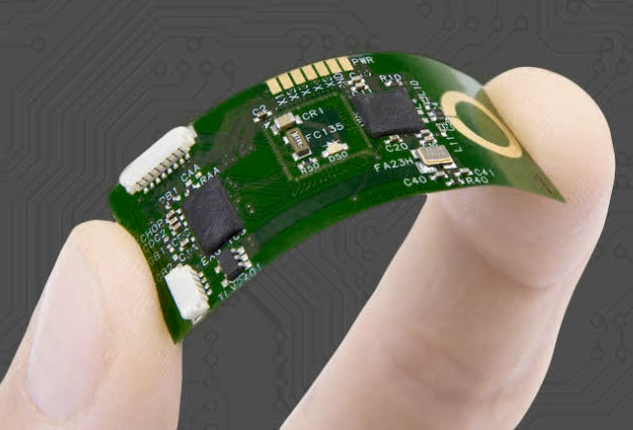
\includegraphics[height=0.2\textheight, width=.8\textwidth]{OBC/AcubeSAT-OBC-G-009_No2/assets/flex.jpg}
			\label{fig:sub2}
		\end{subfigure}
		\begin{subfigure}{.3\textwidth}
			\centering
			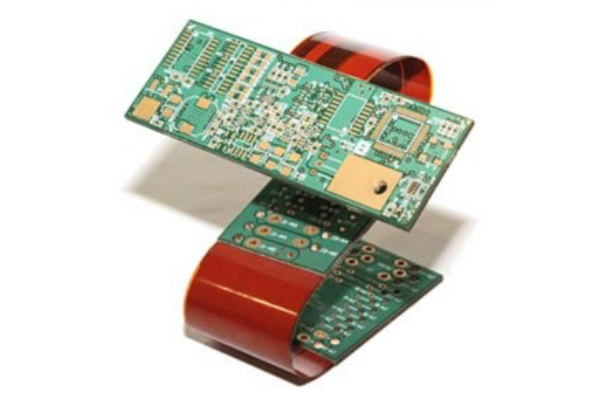
\includegraphics[height=0.2\textheight, width=.8\textwidth]{OBC/AcubeSAT-OBC-G-009_No2/assets/rigid_flex.jpg}
			\label{fig:sub2}
		\end{subfigure}
		\caption{Rigid, flex and rigid-flex PCBs}
		\label{fig:test}
	\end{figure}
	
	If you have been a little bit confused about PCBs…don’t worry! Keep reading and I hope that the following examples will help to make  the situation clear! From now on, we will be focused on simple and common rigid PCBs.
	
	\subsection{Layers}
	
	Printed Circuit Boards can be divided into layers. The increasing technological demands result to multi-layer boards and the stack up (the arrangement of copper layers and insulating layers that make up a PCB prior to board layout design)  is a very important factor. The number of layers range typically from 1 to 16 (\href{https://en.wikipedia.org/wiki/List_of_integrated_circuit_packaging_types}{some} claim that 100-layer PCB is even possible to fabricate!) and usually, in the industry, even numbers are used (2,4,6,8 layers, but single-sided is an exception!). 
	
	Notes:
	\begin{itemize}
		\item 2-layer PCBs called also double sided and 1-layer called single-sided
		\item Using the term layers we are referring to the number of copper layers
	\end{itemize}
	
	Now, let’s examine the layers of the figure 5 that illustrates a fundamental 2-layer PCB: 	
	
	\subsubsection{2-Layer}
	
	\begin{figure}[h!]
		\centering
		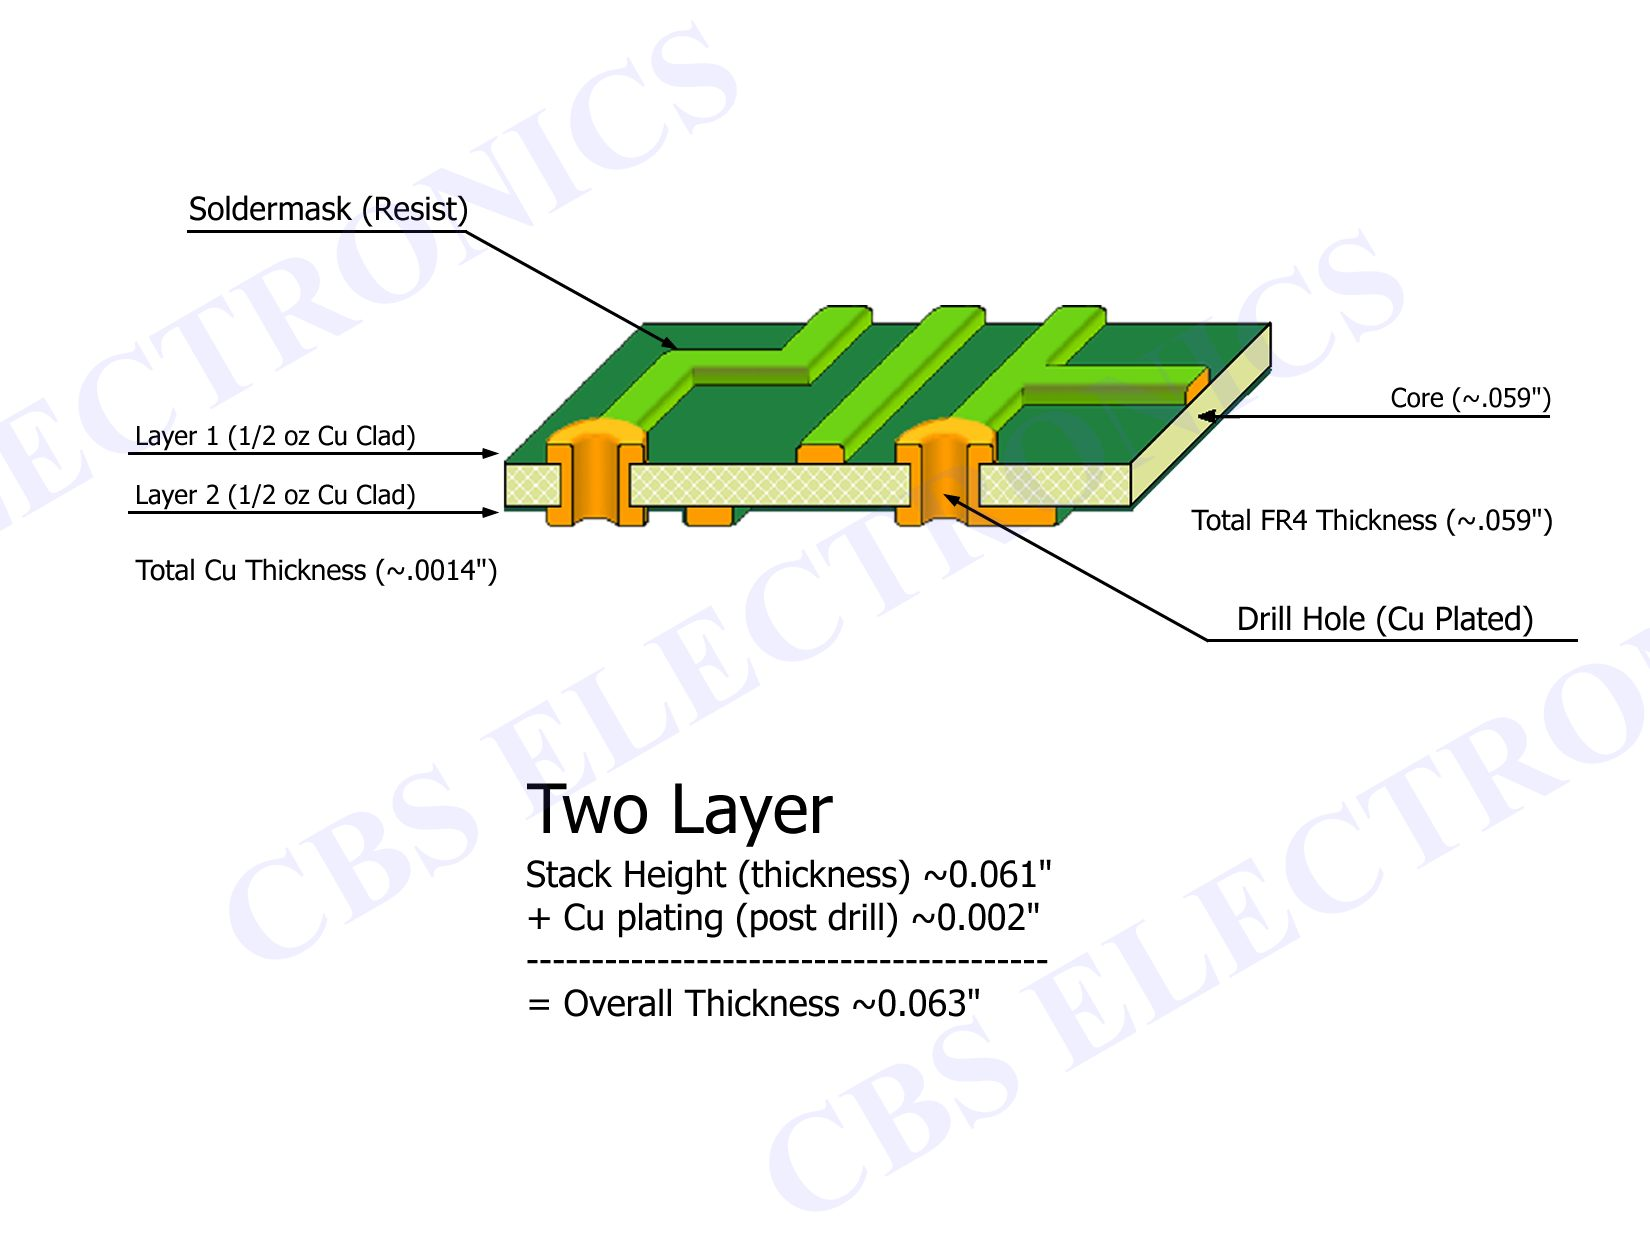
\includegraphics[height=0.45\textheight, width=\textwidth]{OBC/AcubeSAT-OBC-G-009_No2/assets/2lyr_stackup.jpg}
		\caption{}
		\label{fig:my_label}
	\end{figure}
	
	A 2-layer board can be described as a laminate (what holds the layers together, typically FR-4. In this figure the laminate is actually the core) that is coated to the top and bottom side with copper. 
	
	On these copper sides, the routing takes place. The traces (copper paths) are shaped and they serve as the channel for the interface between electrical components. In other words, the point of the copper is to carry electrical signals to and from the PCB, much like your nervous system carries signals between your brain and your muscles. Now, you may be wondered, how it is possible traces that belong to different copper layers to be connected with each other? The answer is via (vertical interconnection access) and it is applied also to multi-layers (I think that the below figure is  explanatory!) 
	
	\begin{figure}[h!]
		\centering
		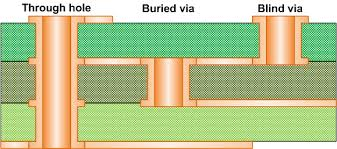
\includegraphics{OBC/AcubeSAT-OBC-G-009_No2/assets/via.jpeg}
		\caption{}
		\label{fig:my_label}
	\end{figure}
	
	About the core, it is a non-conductive substrate usually made of fiberglass. Fiberglass is used because it provides a core strength to the PCB and helps resist breakage. Think of the substrate as the PCB’s “skeleton”. 
	
	\subsubsection{4-Layer}
	Now, that we have a basic understanding about a 2-layer PCB, let’s jump to a 4-layer one:
	
	\begin{figure}[h!]
		\centering
		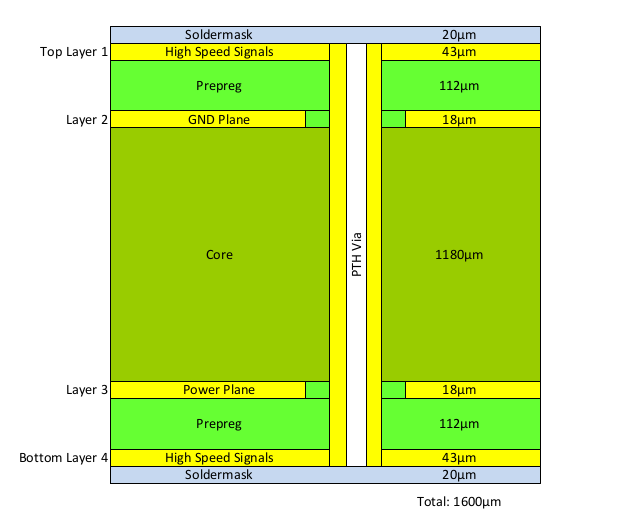
\includegraphics[height=0.3\textheight]{OBC/AcubeSAT-OBC-G-009_No2/assets/4_Layer_PCB.png}
		\caption{}
		\label{fig:my_label}
	\end{figure}
	
	The multi-layer layers are basically a set of 2-layer boards “glued” together and this is also the main reason why even numbers are used. Furthermore, lamination is the process by which the core(s) of a printed circuit board are melted together through heat and pressure with copper layers and prepreg layers (in multi-layer PCBs). In other words, it is the process that creates a “sandwich” or multiple “sandwiches” connected together. It requires specific heating and pressure for specific periods of time based on materials used to ensure the PCB is made properly.  These laminates and the copper thickness comes in different sizes, too.
	
	\begin{figure}[h!]
		\centering
		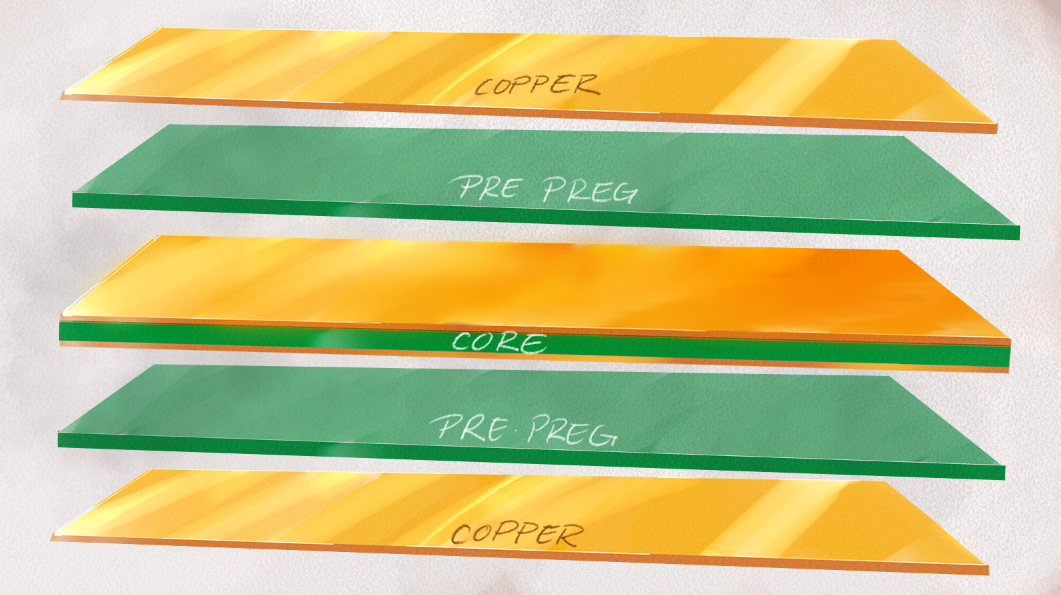
\includegraphics{OBC/AcubeSAT-OBC-G-009_No2/assets/multi-layer-lamination.png}
		\caption{}
		\label{fig:my_label}
	\end{figure}
	
	Noticeable differences between the figure 5 and figure 7 are: 1) the height is the same to these boards (0.063 inches = 1.6 mm) and 2) the new term called \textbf{prepreg}. Someone could say, how it is possible for the overall thickness to be the same in 2 and 4 layers PCB. It’s because laminates and copper foils of different thickness are used to prevent increasing the height of it as the layers are increasing. So a 4-layer board is actually a set of two 2-layer boards separated by  the core, but the overall thickness is the same with a 2-layer design, because in the 4 layer-design the pairs have smaller thickness. A rule of thumb is to have the same thickness above and below of the core! (multi-layers boards can be mirrored). More info about the stack-up thickness can be found \href{https://www.cbspcb.com/pcboard-stackups/}{here}. A prepreg (pre-impregnated) is one of the main materials used in multi-layer boards and is what holds the cores together. It is composed of fiberglass impregnated with resin (an epoxy-based material). The prepreg and core quite often get mixed up (\href{https://electronics.stackexchange.com/questions/356063/what-exactly-is-prepreg-and-core-in-a-pcb}{explanation}). However, they are two separate components of the PCB. The core of the PCB is the FR-4 layers of copper traces and glass-reinforced epoxy laminate sheets. Once heated (lamination) the prepreg holds the core of the PCB and the layers together.
	
	\subsection{Complementary materials/layers}
	\label{subsec:complementary}
	
	Except the fundamental copper layers and the substrate that partitions these layers, there are some other complementary processes during manufacturing that can be defined as extra layers (note: the term layers is used quite a lot and can have several meanings) and they are very useful and necessary nowadays. These are the soldermask, the surface finish/treatment and the silkscreen.
	
	\pagebreak
	
	\begin{figure}[h!]
		\centering
		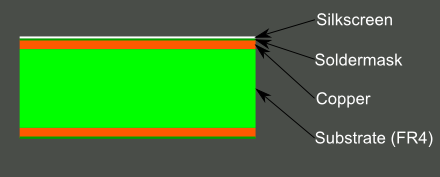
\includegraphics{OBC/AcubeSAT-OBC-G-009_No2/assets/2_layer_plus_silkscreen.png}
		\caption{}
		\label{fig:my_label}
	\end{figure}
	
	\subsubsection{Soldermask}
	
	If you ever wonder why most of the PCBs have a green color in the surface, then now you will understand that the soldermask is the reason! But what it is?
	It is primarily used for protection from oxidization and contact with external environment as well as electrical isolation on the printed circuit board. In addition to benefits as mentioned above, solder mask material also protects from scratching effects of movable electronics parts and thermal aging. The solder mask material is dependent on applications for which particular PCB is manufactured, and also it includes physical dimensions of PCB, size of holes and components. Standards should also be taken into account for which PCB is made whether they are for aerospace or medical or general electronics or telecom industry. Most commonly used material is epoxy liquid material. It had minimal cost and made of polymer type material which is thermal resistant, and it often requires curing thermally. Finally about color, solder mask material comes in different colors, but the most popular material color is green color due to its easily distinguishable color among other electronics and mechanical components and less irritation to the human eyes. Different colors include black, white, yellow, red and orange. Except from the colors, there are also different types of soldermask (check \href{https://www.allpcb.com/soldermask/soldermask_types.html}{this}).
	
	\subsubsection{Surface finish/treatment/coating}
	
	A PCB surface finish is a coating between a component and a bare board PCB. It is applied for two basic reasons: to ensure solderability, and to protect exposed copper circuitry. As there are many types of surface finishes, selecting the right one is no easy task, especially as surface mounts have become more complex and regulations such as RoHS and WEEE have changed industry standards.
	
	For decades HASL (Hot air solder leveling) was one of the most popular surface finish choices. Yet, in recent years, manufacturers have realized its limitations. While a surface finish may be low cost and robust, fundamental changes in the PCB industry—namely, the rise complex surface mount technology—have exposed its shortcomings. HASL leaves uneven surfaces and is not suitable for fine pitch components. Although it does come in lead-free, there are other lead-free options which will likely make more sense for a high-reliability product
	
	ENIG (Electroless Nickel Immersion) is quickly becoming the most popular surface finish in the industry. It’s a double layer metallic coating, with nickel acting as both a barrier to the copper and a surface to which components are soldered. A layer of gold protects the nickel during storage. ENIG is an answer to major industry trends such as lead-free requirements and rise of complex surface components (especially BGAs and flip chips), which require flat surfaces. But ENIG can be expensive, and at times can result in what is commonly known as “black pad syndrome,” a buildup of phosphorous between the gold and nickel layers that can result in fractured surfaces and faulty connections. 
	
	%(maybe put Prisma claiming when sending email)
	
	\subsubsection{Silkscreen}
	
	Silkscreen has no electrical purpose and is usually white and human readable letters, normally used to identify components, test points, PCB part numbers, warning symbols, company logos, date codes and manufacturer marks. This, in turn, makes it easier for electronics assemblers to place each PCB in the proper place and in the right direction on each component. It gives a more artistic tone in the PCB, too!
	
	%(maybe I can put the silkscreen layer of the OBC PCB)
	
	\subsection{Assembly}
	
	It is worth mentioning that the PCB is only the board itself and not the board with the electrical components placed/mounted on the board! The process that is responsible to place the components in the board is called assembly (PCBA: Printed Circuit Board Assembly). Assembly can be done by hand or by machines, called “pick and place”. The soldering and the solderpaste are included in this step. \textbf{Solderpaste} is the material that mounts the electrical components to the surface of the PCB. It’s the link between them. Generally, it is made of a thin-lead alloy, with possibly a third metal alloyed. It is related with the surface finishing, because the last one affects its performance.
	
	Until now, we have discussed a lot about PCB structure and fabrication. But what about the electrical components that can be placed on them. What are the prerequisites? What are the form factors? Why to choose the one or the another?
	
	\subsection{Electrical components/packages}
	
	Most electronic components come in standardized packages. A package type has well a defined set of physical dimensions that the component has to conform to. For each package, normally the pitch spacing, height and general shape is defined. However most packages contain variants with a differing number of leads (for example the classic old-school DIP package comes in 4, 8, and 10 lead variants just to name a few). This means that total land area and size of a package can vary according to how many leads it has.
	Standardizing components sizes and shapes makes it easier for the component manufacturer, the PCB manufacturer, and the design engineer. Although most components are standardized, there are still plenty of packages out there. This pages purpose is to hopefully make some sense of the most common and widely used packages and to help anyone choosing a component package or designing a PCB.
	In general, they can be divided in two main categories: 1) SMT (Surface Mount Technology) and 2) Through-hole, but if you are curious about the packages, you can check the \href{https://en.wikipedia.org/wiki/List_of_integrated_circuit_packaging_types}{well-organized list from wikipedia}! It is worth mentioning that the trend is to be everything SMT.
	
	
	\subsection{Summary}
	
	There are four main parts that characterize a PCB: copper layers, substrate, solderpaste, silkscreen. The essential are copper layers and substrate. The other two act like “helpers” to satisfy some needs in terms of reliability, durability and fabrication. Copper is the channel for the interface between electrical components and the substrate (common material is FR-4) is the base that holds the PCB in one unit. In assembly the Printed Circuit Board is populated (or "stuffed") with electronic components to form a functional printed circuit assembly (PCA), sometimes called a "printed circuit board assembly" (PCBA). Finally, those electrical components come in various packages.
	
	\subsection{Learning resources} %about PCB fabrication
	
	\begin{itemize}
		\item \href{https://www.youtube.com/watch?v=ljOoGyCso8s&t=311s}{JLCPCB}
		\item \href{https://www.eurocircuits.com/making-a-pcb-pcb-manufacture-step-by-step/}{Eurocircuits} + \href{https://www.youtube.com/watch?v=sIV0icM_Ujo&t=436s}{bonus}
		\item \href{https://www.pcbcart.com/article/content/PCB-manufacturing-process.html}{PCBChart}
	\end{itemize}
	
	\section{PCB Design Guidelines}
	
	So now that we have demystify the PCB manufacturing process, let’s start designing a PCB. But why PCB design require thought and why there are so many PCB books describing challenges and potential problems? It isn’t just routing some traces? It isn’t just connected pins? Isn’t SPICE or other electrical simulations tool always right? 
	
	Most people treated printed circuit boards as totally passive devices for connecting components together. As long as the traces were connected to the correct pins, boards almost never had a negative impact on circuit performance. In more recent years, this is becoming less and less true. Many board designers now need to worry about the parasitic elements of traces (resistance, capacitance, and inductance), the interaction between individual traces, and even the interaction between traces and the outside world. 
	
	But what is the main source that causing problems? PCBs carry traces. Traces carry electrical signals that can be digital or analog. Digital and analog signals are flows of electrons that are going back and forth and the main problem is exactly the properties of this oscillation. Electrical current shows its true nature (“transforms”) when it is alternating (AC) and electromagnetic fields are now introduced. Interference and unwanted coupling between conductors have risen to the surface! But we don’t need to panic, because this “transformation” of electrical current is the source of antennas and wireless communications. So, it’s not the “transformation” the problem. The problem is to identify and control it as the designer desires… 
	
	\subsection{How can we identify PCB designs?}
	
	The PCB design can be divided in low-speed, RF and Microwave design. The parameter that separates these topics is the frequency and more specific the rising and the falling time (you will understand why soon). The PCB industry considers any board that operates above 100MHz to be an RF PCB. Anything about 2GHz is a Microwave PCB. But this isn’t strictly defined and problems may occurred when you don’t consider high-speed guidelines even in frequencies that are categorized as low-speed. Theoretically, frequencies at which energy from an oscillating current can radiate off a conductor into space as radio waves starts from 20KHz (RF). Another reference from Texas Instruments (a well known semiconductors industry) claims “With respect to switching output signals, basically, only worry about signals that make an edge transition at a rate greater than 50 kHz. If a pin changes its state at a rate of less than once per 100 instructions, this is acceptable because the contribution from switching is negligible. ”.  Eagle (CAD tool to design PCBs) Academy also claims that “To put it simply, high speed PCB design is any design where the integrity of your signals starts to be affected by the physical characteristics of your circuit board, like your layout, packaging, layer stack up, interconnections, etc… If you start designing boards and run into problems like delays, attenuation, crosstalk, reflections, or emissions, then congratulations! You’ve found yourself in the world of high speed PCB design”.
	
	As mentioned before, the source that causing problems is the nature of oscillating current and its uncontrolled properties. But it’s not only the fact that the current oscillates. The most important factor is how fast it oscillates. In order to start making things clear, it is time to mention the effect of the rising and falling times when a signal is oscillating. Rise time is normally defined as the length of time required for the waveform to rise from the 10\% point on the waveform to the 90\% point.
	
	What is not often stated, but is just generally understood, is that frequency refers to a specific sinusoidal waveform, not something more complex. So when we say the impedance of a circuit is such- and-such a value at 1 MHz, we mean at a 1-MHz sine wave, not, for example, a 1-MHz square wave. That, then, means that when we analyze the performance of a circuit (using the basic formulas) we can do so only at a specific frequency and for a specific waveform (sinusoidal). This raises an interesting question: How do engineers analyze circuits when there are more complex waveforms? The answer is the magical tool called \textbf{Fourier transform}. 
	
	Digital logic circuits deal with signals that look a lot like square waves. \textbf{If we put a square wave onto a trace at one end, we want to get a square wave at the other end}. That means our boards must be designed to handle not only the fundamental frequency of our digital signals, but also all of the higher order harmonics that are contained within it. If we want to be able to handle at least the tenth or fifteenth harmonics. So if we are dealing with a 10-MHz clock square wave, we need to be able to handle frequency harmonics up to at least 100 or 150 MHz. This is why we say it is not the (clock) frequency that matters, it is the rise time of the waveform and the harmonics needed to reproduce it that are important. In conclusion, the faster the rise time, more harmonics are required for integrity. 
	
	The term \textbf{bandwidth} is used to describe this requirement. The bandwidth is the range of frequencies we need to be able to deal with to faithfully maintain the integrity of our signals. Otherwise, bandwidth can be defined as the highest sine wave frequency component that is significant in a signal.
	
	\begin{figure}[h!]
		\centering
		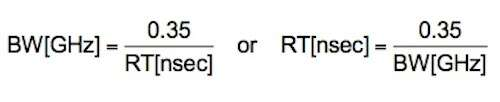
\includegraphics[width=\textwidth]{OBC/AcubeSAT-OBC-G-009_No2/assets/bandwidth_rising_time.jpg}
		\caption{Calculation of Bandwidth}
		\label{fig:my_label}
	\end{figure}
	
	Having these values in our mind we are able to make correct choices when designing the PCB and choosing suitable electrical components (e.g. filters).
	
	\subsection{Signal Integrity issues}
	
	At what point does signal integrity become a problem? For board designers, the answer is: When the rise time decreases to the point where the parasitic inductance and capacitance on the board begin to result in noise signals and transients that become troublesome. 
	
	In general, signal integrity problems on circuit boards fall into four areas, all of which are related to rise time (or related frequency harmonics). They are:
	
	\begin{itemize}
		\item \textbf{E}lectro\textbf{M}agnetic \textbf{I}nterference (radiations beyond the board or susceptibility to radiations from outside the board)
		\item \textbf{Crosstalk} between two or more nets, in
		many ways a special case of EMI
		\item \textbf{Reflections} on a single net
		\item \textbf{Power system stability} during component switching
	\end{itemize}
	
	\subsubsection{EMI}
	
	In one sense, all of our traces are antennas since we are talking about alternating current. A good transmitting antenna is also a good receiving antenna. Therefore, any trace that is a good "radiator" is also a good receiver. Designs that emit EMI are also more susceptible to EMI. In this chapter we will look at design techniques that help reduce EMI. We will see later that the very same techniques also help minimize crosstalk.
	
	\textbf{Identify return current paths}
	
	Around any wire or trace carrying a current, there will be an electrical field (often designated by the letter E) and a magnetic field (often designated by the letter H). Together, these two fields form an electromagnetic field. Now consider that there are two conductors, one with current coming out of the page and one with current going into the page. If these two wires are carrying a signal and its return current, then the currents will be equal and opposite. Therefore the magnetic fields will also be equal and opposite. If the wires were very close together, their EMI radiations would completely cancel and would not be measurable. Herein is one of our most basic principles: \textbf{If you want to minimize EMI radiation, keep the signals and their returns close together}. That, of course, may be easier to say than to do.
	
	\begin{figure}[h!]
		\centering
		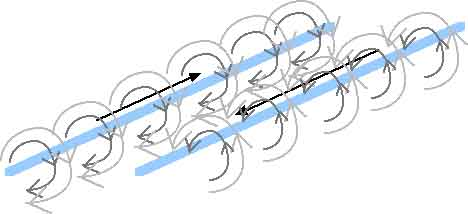
\includegraphics{OBC/AcubeSAT-OBC-G-009_No2/assets/conductor_fields.jpg}
		\caption{EM fields f conductors with opposite current}
		\label{fig:my_label}
	\end{figure}
	
	This is why wires formed into a twisted pair work fairly well in AC environments.
	
	There are a few truths you should always keep in mind. The first, and perhaps most important, is that current always flows in a closed loop. Remember, current is the flow of electrons, and if current does not flow in a closed loop, where do the extra electrons come from or go? Because we know we don't have to deal with buildups of stray electrons on our boards, it seems reasonably intuitive that currents really do flow in a closed loop. That means every signal has a return, somewhere. And you (as the designer) need to know where that is. It sometimes amazes us to discover that designers spend an inordinate amount of time worrying about, considering, and strategizing about 50\% of the signals, and then leave the other 50\% (the return signals) somehow to chance. So the first truth is that every signal has a return and you need to worry about and control where it is. A second rule is that the return current will always follow the path of least impedance. We all have heard the rule that signals follow the path of least resistance, but that is a special case, not the general one. It only applies to low-frequency signals. The general rule, for all signals, and particularly the high-speed signals we worry about, is that return currents follow the path of least impedance (this may not always be where you think it is). In high-speed design, the path with the least impedance is exactly under the trace, provided that a plane exist below the trace layer (to find out more about planes check \autoref{subsubsec:plane})!
	
	\begin{figure}[h!]
		\centering
		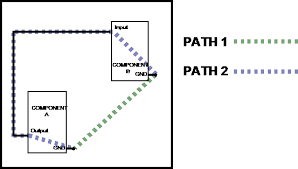
\includegraphics[width=0.7\textwidth]{OBC/AcubeSAT-OBC-G-009_No2/assets/return_current.png}
		\caption{Which path does the signal return current take?}
		\label{fig:my_label}
	\end{figure}{}
	
	\begin{figure}[h!]
		\centering
		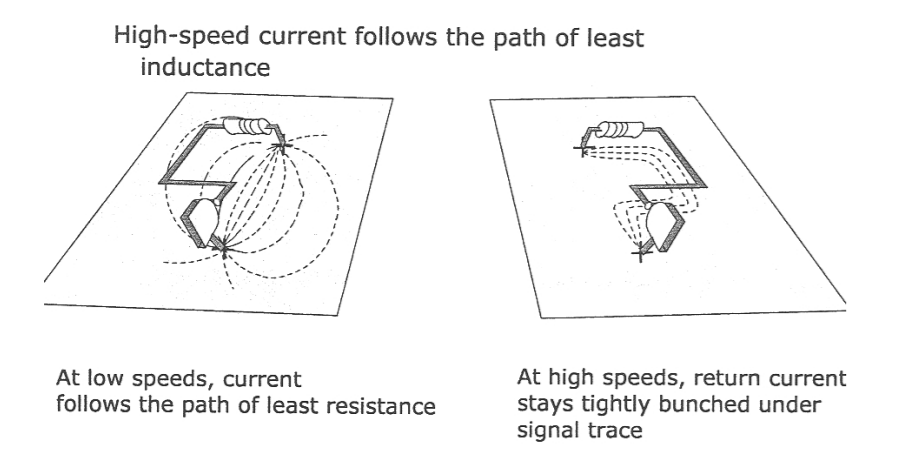
\includegraphics[width=\textwidth]{OBC/AcubeSAT-OBC-G-009_No2/assets/high_speed_return_current.png}
		\caption{Return signal in high-speed}
		\label{fig:my_label}
	\end{figure}
	
	To understand how important is to identify return currents consider the following example:
	
	Let’s assume that we have a trace layer and a ground plane as the figure 14 implicates. If there is a slot in the ground plane, then it will affect the return current path. But what might cause a slot or discontinuity in a plane? Perhaps you have finished the design and then your engineer comes to you with "one more little part" that needs to be added. Making provisions for the routing of this new part may involve a significant amount of rerouting of already routed nets. But, perhaps you could just put a little slot in one of the planes, route one or more of the new traces in that slot, and finish the board quickly. Or, perhaps the plane has been partitioned in some way, creating a discontinuity. Or, perhaps there is a special component requirement nearby that results in a small discontinuity. No matter what the cause of this slot or discontinuity, if a high-speed trace is routed over it, the return signal will be unable to travel underneath that trace. When the return signal hits the discontinuity, it must travel around it and then come back to its position under the trace again. This trip around the slot or discontinuity creates a loop. Since EMI is related to loop area, you have now created a possible EMI problem where none existed previously.  
	
	On the other hand, sometimes slots are unavoidable/inevitable. So, if you are going to make a slot, try to make it as short as possible!
	
	\begin{figure}[h!]
		\centering
		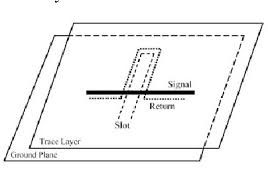
\includegraphics{OBC/AcubeSAT-OBC-G-009_No2/assets/slot_return_current.jpeg}
		\caption{Slot in the return path}
		\label{fig:my_label}
	\end{figure}
	
	\subsubsection{Crosstalk}
	
	Crosstalk is actually a subfield of EMI and it is the unwanted coupling of energy between two or more adjacent lines. This unwanted coupling can change the required signal. So, in this chapter we are going to explain why is this happening and ways to prevent this.
	
	Consider the case where we have two traces adjacent to each other. Current (the flow of electrons) flows down one of the traces (we call this trace the aggressor or driven line). That current will couple into the adjacent trace (called the victim line) and create two different noise signals. One of those noise signals will flow in the victim trace in the same direction as the aggressor current (forward crosstalk). The other noise signal will flow in the victim trace in the opposite direction (backward crosstalk). These two currents have different characteristics and degrees of importance in our circuits.
	
	\begin{figure}[h!]
		\centering
		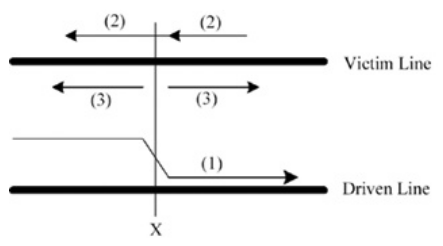
\includegraphics{OBC/AcubeSAT-OBC-G-009_No2/assets/crosstalk.png}
		\caption{Crosstalk}
		\label{fig:my_label}
	\end{figure}
	
	Consider a current (a negative charged net) flowing down the driven line (in Figure 15) and consider an electron as it passes by the specific point X. Electrons are negatively charged particles. Since like charges repel each other, electrons at that point along the victim line will be "repelled" or will move away from point X. They will move in either direction (arrows labeled (3)), so there will be both a backward and a forward component to this reaction. This kind of coupling is almost exactly what we see in capacitors (electrons flowing onto one plate "repel" electrons from the other plate) so this is often referred to as capacitively coupled crosstalk.
	
	The current flowing in the direction of the arrow on the driven line will generate a magnetic field around the line. That field will intersect the victim line and induce (or generate) a current going the opposite direction in the victim line. This mechanism is exactly the same mechanism we find in transformers and in motors and generators. In fact, we can think of the driven and victim lines as being the primary and secondary windings of a poorly designed transformer. The induced current (2) always goes in a direction opposite that of the driven current. We call this induced current inductively coupled crosstalk.
	
	Note that both these mechanisms (capacitively and inductively coupled crosstalk) depend on the fact that the driven current is changing. No coupling occurs if no (or a constant DC) current is flowing. The faster the current is changing (i.e., the higher the frequency or the faster the rise time) the stronger the coupling between the traces. It also seems intuitive that the closer the traces are, the stronger the coupling will be. Already we have two secrets for reducing crosstalk (coupling): Slow down the signals and spread the traces further apart. Another one is the coupling length. So, the shorter the distance that the traces are adjacent, the better in terms of reducing crosstalk. 
	
	A very useful software tool to calculate crosstalk and have specific values is \href{http://www.saturnpcb.com/pcb_toolkit/}{Saturn PCB Toolkit}.
	
	\subsubsection{Reflection and transmission lines}
	
	Consider a long, straight wire or trace with its return wire or trace nearby. The wire has some inductance along its length. There is also some capacitive coupling (a wire that carries electrical current can be though as the thought of a negative charged net) between the wire and its return.
	
	\begin{figure}[h!]
		\centering
		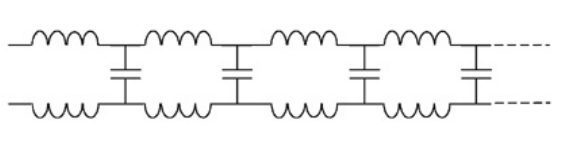
\includegraphics{OBC/AcubeSAT-OBC-G-009_No2/assets/series_inductros_caps.png}
		\caption{Transmission lines as a series of capacitors and inductors}
		\label{fig:my_label}
	\end{figure}
	
	Now, if these wires are infinitely long, there will be no reflection. At least if there is a reflection, it will take an infinitely long time for it to return, so we can assume it doesn't exist. It takes at least one other thing to avoid reflections. The wires must be absolutely-uniform. The little Ls and Cs must be identical everywhere along the wire. If the wires are not uniform, then we can consider them to be multiple sets of wires, each with different characteristics. Individual sets of wires will not be infinitely long, and therefore there will be reflections from each individual set. Therefore, the way to avoid reflections is to use an infinitely long, absolutely uniform wire or trace pair. We give such a wire or trace pair the special name transmission line.
	
	A transmission line of finite length, terminated in its characteristic impedance, Zo, looks like an infinitely long transmission line. Therefore, even though it has a finite length, it still will have no reflections. In this case it is not the infinite length that makes reflections irrelevant. It is the fact that the energy traveling down the line is exactly absorbed (dissipated) in the termination. There is no energy left to reflect back. The net effect is the same thing. There are no reflections to worry about.
	
	
	What actions we need to take to control reflections on PCBs?
	
	We need to make our traces look like transmission lines. We need to terminate them in their characteristic impedance, Zo. Of course, we can also make our traces short enough that reflections don't interfere with the receiver's ability to hear the signal in the first place, or we can slow down the rise time enough that the receiver can hear through the echoes. 
	
	Reflections (echoes) are not too bad a problem if the receiver is close enough to the sender. There is also less of a problem if the message is slowed down (the rise time is slowed down, or lengthened). If we think of a signal traveling down a trace, these two things are actually equivalent. The issue is this: What is the length of the signal path (in propagation time) relative to the rise (or fall) time of the signal?
	
	The general rule of thumb accepted by most people goes like this:
	
	\begin{itemize}
		\item If the propagation time down the trace and back again is less than the rise time of the signal, then we can consider the trace to be short.
		\item If the propagation time down the trace and back again is longer than the rise time of the signal, then we must consider the trace to be long, and we must therefore consider whether terminations might be necessary.
	\end{itemize}
	
	The boundary between these two lengths is called the critical length and is often defined as the length where the two-way delay of the line is less than the rise time of the pulse.
	
	What causes reflections and what do they look like? If we construct our traces to look like transmission lines, we call them controlled impedance traces. We then should be able to control reflections. But if we don't control them correctly, reflections may still exist. The question is why and how large might they be. If we have (tried to) use controlled impedance traces (transmission lines), at least two things might still cause a reflection in the system: (a) an impedance discontinuity along the line, and (b) an improper termination. Recall that the characteristic impedance of a transmission line is defined by its geometry (and the dielectric coefficient of the material surrounding the line). Any change in the geometry, or in the dielectric coefficient, will cause a change in the characteristic impedance of the line at that point. That may (and probably will) cause a reflection at that point. It is imperative that the geometry of our transmission lines be held constant everywhere along the line.
	
	
	\textbf{Impedance discontinuity} can happen when:
	
	\begin{itemize}
		\item \textbf{Changing Trace Layers}
	\end{itemize}{}
	
	
	Since the environment often changes when we change layers, we usually have to also adjust the trace width when we change layers. This is necessary because what is important is maintaining a constant impedance (not just a constant geometry) on each layer. If we are designing with a certain impedance in mind (say 50 W) we have to determine what a 50-W trace looks like on each layer of our board. Then, if we move a 50-W trace to that layer, we may have to change the trace's properties to maintain the desired impedance on that particular layer.
	
	\begin{figure}[h!]
		\centering
		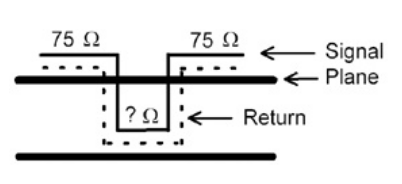
\includegraphics{OBC/AcubeSAT-OBC-G-009_No2/assets/changing_layers_trace.png}
		\caption{Changing trace layers}
		\label{fig:my_label}
	\end{figure}
	
	\begin{itemize}
		\item \textbf{Slots in planes}, as have been described previously
		
	\end{itemize}
	
	\subsubsection{Power stability}
	\label{subsubsec:plane}
	
	Schematic diagrams have wires, but in real life there are no wires (unless someone has started manufacturing PCBs using superconductors...). Physical interconnects, including PCB traces, are low-value resistors (\textbf{Copper Is a Resistor}). The fact that we can often ignore this interconnect resistance doesn’t mean that it has no effect on the functionality of a circuit. Power and ground traces carry usually high currents and if we don’t take into account the impedance of these traces, then we will end up with significant voltage drops and some components may not receive the proper differential voltage in order to function. This is why we use mostly planes (or wider traces) for power and ground traces. Planes are  are large areas of copper foil that are connected to either a power supply potential or the common connection (ground)  and serve as low impedance paths.
	
	When multiple supply voltages are used on a PCB, then special considerations should be taken. How many planes should
	I use? What should be on them? Where should they be placed?
	
	For example, every different power supply voltage is typically distributed on its own plane. It is logical that each different regulated supply of the same voltage also gets its own plane; otherwise some of the regulated supply sections would simply be shorted out. Very often, however, all the different regulated supplies are referenced to the same voltage potential​ zero volts. Is it possible, then, to have only one ground plane (at zero volts) that can service all the individual regulated power supplies, or do we need a separate ground plane for each individual regulated supply?
	
	It may be perfectly fine for two supplies to reference the same ground plane. In some cases, a circuit simply involves two types of ICs with different supply requirements, and a single reference (zero-voltage) plane may work well here, too. And, if we have mixed signals (as in an A/D circuit) but all the circuits are known to be quiet, so noise is not a concern, a single reference plane might be adequate. 
	
	\begin{figure}[h!]
		\centering
		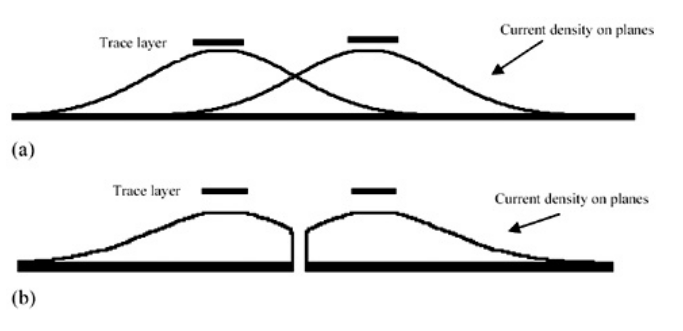
\includegraphics[width=\textwidth]{OBC/AcubeSAT-OBC-G-009_No2/assets/different_planes.png}
		\caption{}
		\label{fig:my_label}
	\end{figure}
	
	If circuit noise is our primary focus, then we almost always need to define separate reference (ground or zero-voltage) planes for each individual regulated supply section. Consider the implications for not doing so. Assume, in a transmitter section, we send a signal down the trace shown in Figure 18- a. The return signal, although primarily underneath the trace, extends for
	some distance beyond the edges of the trace. If any receiver circuitry is anywhere near this return gradient, some of this transmitter noise may couple
	into the receiver section. In addition, there are current gradients that flow
	from the transmitter-regulated power supply across the ground plane while charging (and discharging) any bypass capacitors that may exist. These
	currents may also couple into receiver circuitry. The whole point of having a
	separate receiver power supply section is to try to isolate the two sections. A single ground (reference plane) tends to work against this objective. So, good design practice is to have separate ground planes for the receiver and
	transmitter sections (Figure 18-b).
	
	
	\subsection{PCB Layout Techniques}
	\label{subsec:techniques}
	
	Some additional techniques to handle properly the signal integrity issues that described in the previous subsection!
	\subsubsection{Stack-up}
	First of all we are going to summarize the importance of planes in PCB.
	\begin{itemize}
		\item \textbf{Impedance control}: If we want to control trace impedance as a strategy for the control of reflections (using proper trace termination techniques), then good, solid, continuous planes are almost always required. It is very difficult to control trace impedance without the use of planes.
		\item \textbf{Loop areas}: Loop area can be visualized as the area defined by the path of the signal (traveling down a trace) and its return current. When the return signal is on the plane immediately under the trace, loop area is minimized. Since EMI is directly related to loop area, EMI is minimized when good, solid, continuous planes exist under traces.
		\item \textbf{Crosstalk}: The two most practical ways to control crosstalk are (a) separation between traces and (b) closeness of the traces to their reference planes. Crosstalk is inversely proportional to the square of the distance between the traces and their reference planes.
		\item For Plane Pairs
		\begin{itemize}
			\item Decoupling: The capacitance formed by the proximity of two planes placed close together can be very important and beneficial in circuit decoupling at very high frequencies, where bypass capacitors and their associated mounting and lead inductance begin to have problems.
			\item EMI: Planar capacitance can be effective in controlling EMI radiations caused by both differential mode and common mode noise signals.
		\end{itemize}{}
	\end{itemize}
	
	
	Stack up is the arrangement of copper layers and insulating layers that make up a PCB prior to board layout design. Planes, as we have already understand, are quite efficiently and this one of the main reasons that someone is going to use a multi-layer design. We need to understand that each type of stack-up should be relevant with the designer priorities. There isn't a generic best stack-up, it is application-dependent. 
	
	\href{http://www.hottconsultants.com/techtips/pcb-stack-up-2.html}{Here} you can see an explanation of different stack-ups in a 4-layer desing
	
	Finally, a very interesting \href{https://www.pcbcart.com/article/content/factors-determining-PCB-layers.html}{reference} claims that \textbf{4-layer} designs are mostly used in \textbf{satellite systems} (just a reference though, without details).
	
	\subsubsection{Copper fill/pour}
	In 2-layer designs is quite common to use copper fills to somehow create a plane. This technique isn't as efficient as using a solid plane, though. Copper fills are applied to signal layers where the empty area left from traces is filled with copper connected to the power or ground potential.
	Copper fills are also used to multi-layer design, in the signal layers. This is happening, because the bigger the copper area the less the impedance. The only thing left to do is to connect these copper areas with vias.
	
	\subsubsection{Vias stiching and Via shielding}
	Via stitching is a technique used to tie together larger copper areas on different layers, in effect creating a strong vertical connection through the board structure, helping maintain a low impedance and short return loops. Via stitching can also be used to tie areas of copper that might otherwise be isolated from their net, to that net.
	
	Via shielding has a different function, in RF designs it is used to help reduce crosstalk and electromagnetic interference in a route that is carrying an RF signal.  A via shield, also known as a via fence or a picket fence, is created by placing one or more rows of vias alongside the signal's route path. In Altium Designer, this is referred to as via shielding.
	\subsubsection{Partitioning the design}
	%the same things applies for the planes as discussed for the power stability
	The schematic of almost any electronic application is a concatenation of functional blocks. It is essential that those blocks are correctly identified and that the components within each block are grouped together on the PCB, in order to minimize crosstalk and reduce interconnections length. Most signal integrity problems associated with high speed signals can be addressed by propped component placement. Prior to detailed placement and routing, the schematic should be partitioned into functional blocks. Furthermore, to ease the next step of zoning, the functional blocks should be classified according to the specificity of the signals contained.
	
	\begin{figure}[h!]
		\centering
		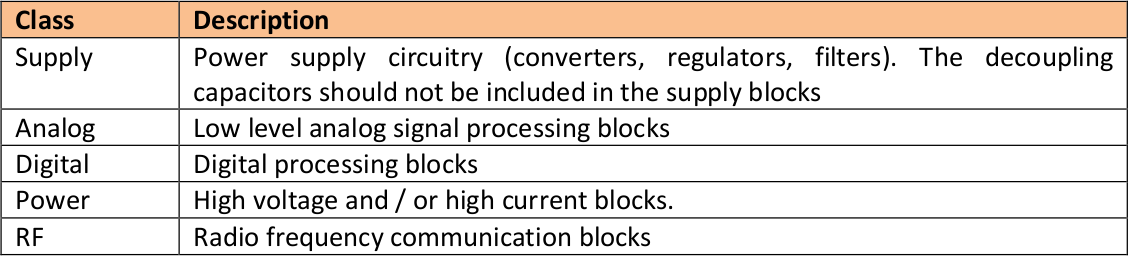
\includegraphics[width=\textwidth]{OBC/AcubeSAT-OBC-G-009_No2/assets/partitioning.png}
	\end{figure}{}
	
	Once the system is partitioned into functional blocks, each should be assigned a distinct physical location on the PCB. This operation is called “zoning” or “floor-planning”. 
	
	A draft placement should be made in order to estimate the space necessary for each block. The zoning should tend to minimize the length of the interconnections between blocks and also the electromagnetic coupling between them. Coupling can be caused either by electromagnetic fields interference, which can be minimized by physically placing the blocks as far apart as possible, either by common impedance, which is caused by return currents following the same physical path. Since all currents return to the power supply, the common return between each block class should be made as short as possible. This requires the most “aggressive” blocks (RF, Power, Digital) to be placed closer to the Supply and the most sensitive blocks (Analog) to be placed farther to the Supply. If possible, highly “aggressive” blocks (RF) should be isolated from the main circuitry in order to completely avoid a common return path.
	
	Figure 19 presents a recommended zoning for an application with several functional blocks.
	
	\pagebreak
	
	\begin{figure}[h!]
		\centering
		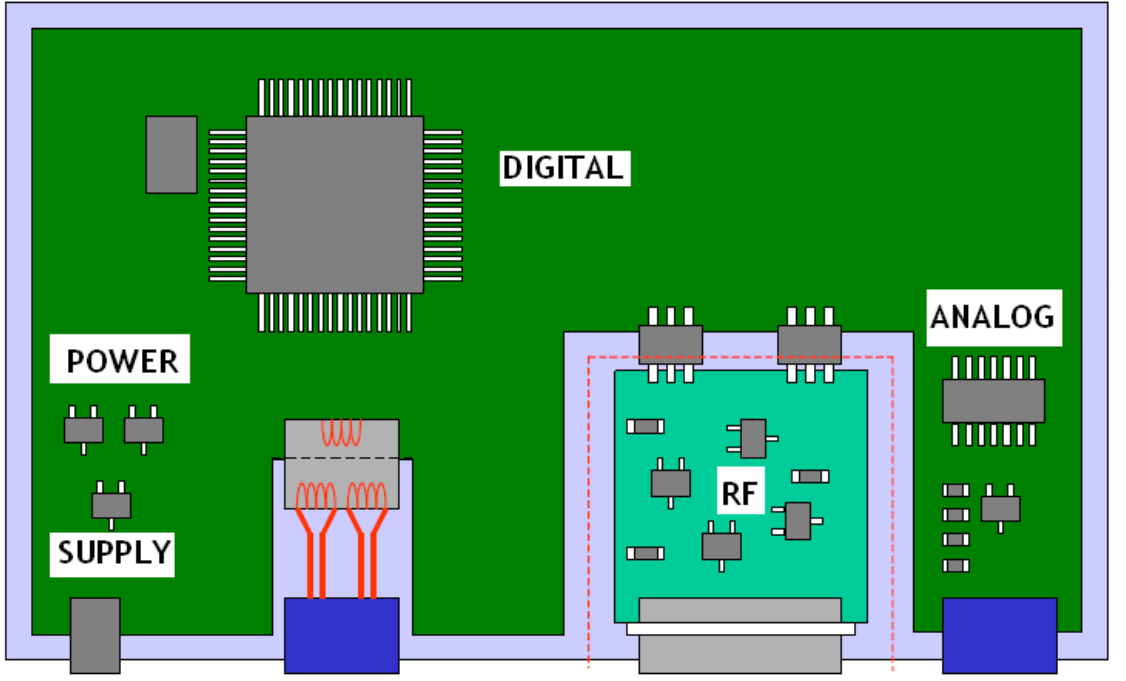
\includegraphics[height=0.35\textheight, width=\textwidth]{OBC/AcubeSAT-OBC-G-009_No2/assets/zoning_example.png}
		\caption{}
		\label{fig:my_label}
	\end{figure}
	
	\subsubsection{Guard band}
	Guard bands are sometimes used to isolate traces from each other. The idea is
	to place a trace, called a guard band, between the aggressor and the victim
	traces. The guard band trace is grounded. Thus, it acts as an electrical shield between the other two traces, much like the shield in a shielded cable might.
	
	The most common application for guard bands is when crosstalk is an issue.
	The idea is that any coupling that takes place will be to ground (the guard
	band) and not into the next, more sensitive signal trace.
	
	Although there is not uniform agreement on this issue, most people feel that
	guard banding is ineffective at best and can actually be harmful at worst.
	There are several issues that can be of concern here. The first is how and
	where to ground the guard trace. It certainly must be grounded at one end,
	but many people say it should be grounded at both ends. The problem with
	this solution is that now the possibility for ground loops has developed. That is,there is the possibility that stray currents may find their way onto the guard trace at one end and propagate down the guard trace and back to ground at the other end. Ground loops can have very serious effects on performance, not the least of which is the creation of EMI problems.
	
	
	\subsubsection{Unused pins}
	Unused input pins should not be left floating, as they might oscillate due to
	electromagnetic interference and increase the dynamic supply current. Unused input pins should be connected to a DC potential, either VCC or GND.
	Unused output pins should be left unconnected Unused bidirectional pins should be configured as inputs and connected to VCC or GND. If they cannot be permanently configured as inputs they should be connected to VCC or GND using a high value resistor. Note that this resistor will act as a pullup or pulldown when the bidirectional pin is configured as input and as a load when the pin is configured as output, so it will determine the current sourced / sunk by the IC.
	
	\subsubsection{Decoupling caps}
	Decoupling capacitors between the power pin and ground pin of the device ensure low AC impedance to reduce noise and to store energy. To reach low impedance over a wide frequency range, several capacitors must be used. This is why, a real capacitor consists of its capacitance and a parasitic inductance and resistance. Therefore, every real capacitor behaves as a resonant circuit. The capacitive characteristics are only valid up to its self-resonant frequency (SRF). Above the SRF, the parasitic effects dominate, and the capacitor acts as an inductor. With the use of several capacitors with different values, low AC impedance over a wide frequency range can be provided.
	
	General rules for placing capacitors:
	
	\begin{itemize}
		\item Place the lowest valued capacitor as close as possible to the device to minimize the inductive influence of the trace. This is especially important for small capacitor values, because the inductive influence of the trace is not negligible anymore
		\item Connect the pad of the capacitor directly with a via to the ground plane. If the distance to the ground pin of the device is short enough,you can connect it directly.
		\item Make sure that the signal must flow along the capacitor.
	\end{itemize}
	
	\subsubsection{Trace geometry/angle}
	
	The most widely used angle for traces is 45 degree. The reasons are that they look cleaner, the 45 degree trace geometry offers a shorter path between components and its common practise.
	
	In general, there is a rumour not using 90 degree angles, because right angles radiate more. But \href{https://electronics.stackexchange.com/questions/226582/pcb-90-degree-angles}{this isn't exactly true}.
	
	\subsubsection{Stubs}
	In Figure 20  current only travels through the via portion between the two traces; the via will typically be very short compared with the overall length of the traces. Below this portion, however, the unused stub, a conductive portion of the via not connected in series with the circuit, presents itself as an unterminated transmission line with significant signal degradation around its resonant frequency (determined by the quarter wavelength of the structure.) The longer the stub, the larger the impedance discontinuity and consequent loss to the signal path. In general, a stub presents significantly more signal degradation than the via itself.
	
	\begin{figure}[h!]
		\centering
		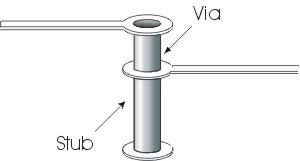
\includegraphics[height=0.3\textheight, width=\textwidth]{OBC/AcubeSAT-OBC-G-009_No2/assets/stub.jpeg}
		\caption{}
		\label{fig:my_label}
	\end{figure}
	
	Stubs generally serve no useful purpose in a circuit so are often removed by back-drilling. Back-drilling (where the undesired conductive plating in the stub section of the via is removed using a drill bit slightly larger in diameter than the drill bit used to create the original via hole) can provide significant improvements, especially if the stub is long. Back-drilling can improve impedance matching and reduce resonance with consequent reduced signal attenuation, reduce EMI/EMC radiation and reduce crosstalk between vias. A full analysis of stub behaviour is possible with 3D full-wave simulation but a rule of thumb commonly employed by many signal integrity engineers is simply to (bypass the time-consuming analysis and) make the stub length as short as possible.
	
	\subsubsection{Design for Manufacture}
	
	\textbf{Component orientation}
	
	Whenever you place like-minded components on your board, like a set of resistors or LEDs, it would be nice to facing the same direction. Why? This will make your board much easier to install, test, and inspect by your manufacturer.
	
	The second point to consider is how you are placing your components in relation to each other. When your completed board gets handed off to your manufacturer, they’re going to send it through a soldering oven to connect all of the parts to your bare circuit board. If you have taller components that are blocking smaller ones, then chances are you’ll likely get a board back with poorly connected solder joints. When placing components, always be mindful of their size not just in your two-dimensional space, but also their height and width (\href{https://www.autodesk.com/products/eagle/blog/top-10-pcb-component-placement-tips-pcb-beginner/}{placement tips})
	
	\textbf{Fiducial marks}
	
	Fiducial marks or markers are circuit pattern recognition markers. Basically it is a round solder mask opening with round bare copper in the center. Bare copper has a smaller diameter than the solder mask opening. Pick and place machines use Fiducial marks as referent points on the PCB to position the Surface Mount Components (Packages) on the PCB during assembly of the Printed Circuit Board.
	
	\textbf{Cost}
	
	A very important factor a designer needs to consider is the fabrication cost. For example, in a 2-layer board placing components in the top and bottom layer, will increase the cost significantly. A better solution might be to upgrade to a 4-layer design and keep all the components on the top. With that in mind you will have the advantages of a 4-layer design, in terms of noise, keeping the cost "low". Of course this approach isn't mandatory, just food for thought.
	
	\textbf{DRC}
	
	There are things that the manufacturer is available to do and others that don't (minimum width, minimum clearance etc). The designer, in order to be compliant with the fabrication-abilities there are the so called Design Rules Check. Each EDA, has a DRC tool and it is basically a software test that indicates if some design rules are violated or not. A design rule set specifies certain geometric and connectivity restrictions to ensure sufficient margins to account for variability in semiconductor manufacturing processes, so as to ensure that most of the parts work correctly. 
	
	
	
	
	%\subsubsection{Workflow}
	%\textbf{First route the critical traces}
	
	\subsection{Rules of thumb}
	\label{subsec:thumb}
	
	\begin{itemize}
		\item In general keep traces short and wide
		\item Keep signals and their return paths as close as possible. Avoid slots in planes or keep them short
		\item Be aware of the return current paths and try to visualize how current will flow (easy to say, hard to do!)
		\item Spread unrelated signals as further apart as possible and keep the distance, that these signals are adjacent, short
		\item Slow down the signals (clock frequency) if there is no need of higher frequencies
		\item Provide low-impedance path for the power supply and ground
		%\item Be aware of the sources of EMI and victim. Eliminate the interference and protect the victims!
		\item Identify the vulnerable parts of your PCB design and partition it efficiently. What components are sensitive in power-supply terms? What is the rise time of this data signal? What should I do when mixing analog and digital signals? What precautions should I take?
		\item Impedance control and termination if it is required
		\item Decoupling caps!
		\items Read the datasheets to find any specific required hardware support
		\item Don't forget the manufacturing process and design accordingly to the manufacturer (e.g. orientation of components)
		\item Unused pins should be tied to the ground
		\item Avoid ground loops
		\item Use vias with care
		\item First route the critical traces
		\item An old saying is that PCB design is 90\% placement and 10\% routing.
		\item PCB is art! If it looks good, it will work good!
	\end{itemize}
	
	\subsection{Learning resources}
	\begin{itemize}
		\item[-] Howard Johnson, Martin Graham. High Speed Digital Design: A Handbook of Black Magic 
		\item[-] Peter Wilson. The Circuit Designer's Companion
		\item[-] Mark I. Montrose. Printed Circuit Board Design Techniques for EMC Compliance 
		\item[-] Douglas Brooks. Signal Integrity Issues and Printed Circuit Board Design
		\item[-] \href{https://drive.google.com/file/d/1C4cFAzJpTlKedcgKvlWDQnTaCCgdo58s/view?usp=sharing}{EMC Fastpass. Getting EMC design right at the first time}
		\item[-] \href{https://drive.google.com/file/d/1mr8UNMDeXmdCBnOVq22b1YUi3WwKNUMm/view?usp=sharing}{Texas Instruments. High-Speed Layout Guidelines}
		\item[-] \href{    https://drive.google.com/file/d/1gwrVG8WULKCOxYYrVLvCCZh1-luvQacq/view?usp=sharing}{NXP. High-Speed Layout Guidelines}
		\item[-] \href{https://drive.google.com/file/d/1ylptbGbczsr2scbjPCba7q4J1PiyvQL8/view?usp=sharing}{David L. Jones. PCB Design Tutorial}
		
	\end{itemize}
	
	\section{PCB designing software}
	
	AcubeSAT is currently using KiCad as a CAD tool to design the PCBs. One of the main reasons for this selection is that it is open-source and sufficient good for our jobs. In the PCB industry, the most widely used CAD tool is Altium because it has quite a lot advanced features. But, the choice of CAD tool is individual and based on personal needs/desires. Just for reference, other CAD tools for PCB design are Eagle, OrCAD, gEDA, EasyEDA etc.
	
	
	\subsection{KiCad}
	
	To start learning KiCad, useful resources are the well-written documentation from \href{http://docs.kicad-pcb.org/}{KiCad website} and a detailed book, \href{https://drive.google.com/file/d/1z3XU2MWJjkBjeA_4xKuLXPgRW0tIhxVv/view?usp=sharing}{KICAD LIKE A PRO}. Of course, the best way to learn a tool is start using it!
	
	\subsection{PCB parts database}
	
	Schematic symbols and footprints are necessary parts for your EDA software to design your PCB. Databases for these are \href{https://www.snapeda.com/}{SnapEDA}, \href{https://www.samacsys.com/}{SamacSys}, \href{https://www.ultralibrarian.com/}{UltraLibrarian}. You should be very careful when using ready symbols and footprints, because they may not be just right for your design. So, check them thoroughly!
	
	
	%\textbf{Love & Peace}
	%\section{TODO}
	%\begin{itemize}
	%    \item Amplifiers
	%   \item "Tuning" traces. Signal timing
	%    \item High density interconnection (just for the heck of it)
	%    \item More info about transmission lines
	%    \item Differential signaling, single ended
	%    \item thermal issues/analysis
	%    \item structural things
	%\end{itemize}
	
\end{document}